\documentclass[a4paper, 11pt]{report}
\usepackage[dvipdf]{graphics}
\usepackage{times}
%------------------------------------------------------------------
% Macros used
\newcommand{\subarg}[1]{\textsl{#1}}
\newcommand{\valconst}[1]{\textsl{#1}}
\newcommand{\nonterm}[1]{\textsl{#1}}
\newcommand{\keyword}[1]{\texttt{#1}}
\newcommand{\arrow}{\ensuremath{\rightarrow}}
\newcommand{\switch}[1]{\textsl{#1}}


\begin{document}
\begin{titlepage}

\vspace{2cm}
\center{\Large L98 Compiler}

\vspace{3cm}
\center{Paulo Pinto and Pablo Tavares}
\center{First release, 24 October 1999}
\center{Second release, 14 April 2013}

\end{titlepage}

\tableofcontents

%-------------------------------------------------------------------------
\chapter{Foreword}

This compiler was developed as part of a workgroup project in 1999, while both
of the authors were at the university.

Although the compiler was developed in Java, one of the mainstream languages in
use nowadays, it shows its Java 1.1 roots in several places.

So a decision was made to bring the build infrasture, code generation and overrall
code structure to Java 7, while dropping a few uses that were only relevant in Java
1.1 days.

Additionally the compiler is now GPL licensed.

\chapter{The L98 Language}


This chapter is intended to present L98 to the reader. After reading this
chapter you should be able to write L98 programs without much dificulty.

L98 has a syntax that resembles ML but it is not a funcional language. L98
allows the use of procedures and has I/O like imperative languages. So you
should consider L98 an imperative language.

The language is based in the one described in the book known as the \emph{Tiger
Book} \cite{tiger}.

\section{Types}

As most languages, L98 has data types. Because the language is very simple, it
only posses two data types. The data type \keyword{bool} represents the boolean
values true and false. The data type \keyword{int} represents signed integers.

\section{Statements}

L98 has all the common statements that can be found in current
languages. It has statement for performing loops, like \keyword{for}
and \keyword{while}. It has two statements for performing control
flow, \keyword{if}\dots\keyword{then}\dots\keyword{else} and
\keyword{return}.

\subsection{Simple Statements}

In L98 as in every other language, the assignment is a fundamental
operation, so it is the first statement to be presented. You can assign
values to variables like this:

\begin{verbatim}
someVar    := 2;
anotherVar := 4 + someVar * 2;
aboveTen   := anotherVar > 10
\end{verbatim}

Since we must use variables to store the values of expressions, we
need a way to declare them. In L98 the statement used to declare
variable is \keyword{let} as shown:

\begin{verbatim}
let
  var someVar: int := 0
  var anotherVar: int := 0
  var aboveTen: bool := false
in
 someVar    := 2;
 anotherVar := 4 + someVar * 2;
 aboveTen   := anotherVar > 10
end
\end{verbatim}

Note that every variable must be initialized in the declaration. The
variables can only be used in the \keyword{in}\dots\keyword{end} part
of the \keyword{let} statement.

The L98 uses lexical scope for the variables, as demostrated by:

\begin{verbatim}
let
  var someVar: int := 5
in
 printint (someVar); /* Prints 5 */
 let
  var someVar: int := someVar + 1
 in
  printint (someVar) /* Prints 6 */
 end;
 printint (someVar); /* Prints 5 again */
end
\end{verbatim}

The routine \emph{printint ()} and several others are described in section \ref{sct:builtin}
and appendix \ref{sct:routines}.

\section{Control Flow}

\subsection{Decisions}
Like every available language, L98 must have a way to make
decisions. In L98 the \keyword{if} is available for that
purpose.

The \keyword{else} part of the \keyword{if} statement is
optional.

As an example of the \keyword{if} statement we could make
the following code:

\begin{verbatim}
let
  var someVar: int := 0
  var positive: bool := false;
in
 someVar := readint (); /* Reads an int value from the input */
 if someVar > 0 then
  positive := true;

 /* or */
 if someVar > 0 then
  positive := true
 else
  positive := false
end
\end{verbatim}

\subsection{Performing Loops}
The loops are another form of control flow, that is why they are also in
this section.
In L98 there are two forms of loops. The \keyword{for} loop and the
\keyword{while} loop.

The \keyword{for} loop can be used in two different ways. It could be
a loop in which the control variable gets incremented, or decremented.
The variables used in the \keyword{for} loop don't need to be declared.
To print all the numbers from 0 to 10 we could write something like this:

\begin{verbatim}
for i := 0 upto 10 do
  printint (i)
\end{verbatim}

If we want to print in the reverse order, we could change the loop to
this form:
\begin{verbatim}
for i := 10 downto 0 do
  printint (i)
\end{verbatim}

The \keyword{for} loop is only adequate when we know how many
times to perform the loop. When the loop must be executed while some
condition holds, the soluction is a \keyword{while} loop. To calculate
a factorial using a \keyword{while} loop, we could write something like
this:

\begin{verbatim}
let
  var value: int := readint ()
  var  temp: int := 0
in
  while value > 1 do
   (
     temp := temp * value;
     value := value - 1
   );
 printint (temp)
end
\end{verbatim}

The (\dots) represents a list of statements and is used like the \{\dots\} in C
or \keyword{begin}\dots\keyword{end} in Pascal.


\section{Sub-Routines}
L98 supports the definition of sub-routines. They are defined by the use of
the \keyword{let} statement, and can be functions or procedures.

\subsection{Functions}
As an example let's declare a function to calculate the square of its argument:

\begin{verbatim}
let
  var i : int := 0

  fun square (val x: int): int = return x * x
in
  i := square (2);      /* i contains 4 */
  i := square (3)       /* i contains 9 */ 
end
\end{verbatim}

As you can see, the functions are called as in C or Pascal by using the
name of the function followed by a list of arguments enclosed in (\dots). In
L98 when a function doesn't have any arguments it must be called using an
empty list. let's write a function that acts as a constant and doesn't have
arguments:

\begin{verbatim}
let
  var i : int := 0

  fun const (): int = return 5
in
  i := const ()      /* i contains 5 */
end
\end{verbatim}

Another thing that you should note, is that in the \keyword{let} statement the
declarations and variables must appear before the declarations of sub-routines.

Having the possibility of executing a statement is good, but we want more. How do
we declare a function with several statements? There are several solutions to this
problem. One way is to use a statement list :

\begin{verbatim}
let
  var i : int := 0

  fun const (): int = (i := 2 * 3; return 5)
in
  i := const ()      /* i contains 5 */
end
\end{verbatim}

Or we can use a statement that allows multiple statements, as the \keyword{let}. So
we could arrange the previous code to:

\begin{verbatim}
let
  var i : int := 0

  fun const (): int = let
                      in
                        i := 2 * 3;
                        return 5
                      end
in
  i := const ()      /* i contains 5 */
end
\end{verbatim}

\subsection{Procedures}

Using procedures is as easy as using functions, so you could declare a procedure like this:


\begin{verbatim}
let
  var i : int := 0

  proc test () = i := 5
in
  test ()      /* after the call of test (), i contains 5 */
end
\end{verbatim}

Of course this routine isn't very helpful, so let's create one that outputs the value of
an integer followed by a new line:

\begin{verbatim}
let
  proc printintln (val i: int) = (printint (i); println ())
in
  printint (2);
  printint (3);   /* Prints 23 */
  printintln (2);
  printintln (3)  /* Prints 2
                            3 */
end
\end{verbatim}

\subsection{Multiple Arguments}
Both functions and procedures allow the use of more than one argument,
for that you just have to declare them using a \textbf{;} as separator. As
an example, the sample code for the min function is provided :

\begin{verbatim}
let
  fun min (val a: int; val b:int) = if a < b then
                                      return a
                                    else
                                      return b
in
  printint (min (2,3)) /* Prints 2 */
end
\end{verbatim}

\subsection{Variable Arguments}
Sometimes we need to pass an argument that is modified by the subrotine and
preserves its value after the call. One example of such procedure is one that
exchanges the contents of its arguments, like the following one:

\begin{verbatim}
let
  var x: int := 0
  var y: int := 6
  proc swap (var a: int; var b:int) = let
                                       val temp: int = a
                                      in
                                       a := b;
                                       b := temp
                                      end
in
  printint (x); /* Prints 0 */
  printint (y); /* Prints 6 */
  swap (x, y);
  printint (x); /* Prints 6 */
  printint (y)  /* Prints 0 */
end
\end{verbatim}

The difference is that the arguments are declared with \keyword{var}, as in Pascal.

\subsection{Recursion}

It is possible to use recursion in L98. As an example let's code the
famous factorial using recursion:

\begin{verbatim}
let
  func fact (var x: int): int = if x = 0 then
                                  return 1
                                else
                                  return x * fact (x - 1)
                                      end
in
  printint (fact (2)) /* Prints 2! => 4 */
end
\end{verbatim}

\section{Builtin Routines}
\label{sct:builtin}

There are some routines that are available to all programs in L98. They are used
to read and print the values of the builtin types, and to emit a new line to the output.

The available routines are:

\begin{description}
\item[printint] Takes an integer as argument and outputs its value;

\item[printbool] Takes a bool as argument and outputs its value;

\item[readint] Reads an integer from the input and returns its value;

\item[readbool] Reads a bool from the input and returns its value;

\item[println] Outputs a new line
\end{description}

These routines are fully described in appendix \ref{sct:routines}.
The output and input of the programs in L98 are the standard output and
standard input of the process.

%------------------------------------------------------------------
\appendix

%------------------------------------------------------------------
\chapter{L98 Language Definition}
\section{Keywords}
The table \ref{tbl:keys} sumarizes the available keywords in L98.

\begin{table}[htb]
\center
\begin{tabular}{|c|c|c|c|c|}
 \hline
 \keyword{and} & \keyword{end} & \keyword{in} & \keyword{proc} & \keyword{while}\\
 \hline
 \keyword{bool} & \keyword{false} & \keyword{int} & \keyword{return} & \keyword{val}\\
 \hline
 \keyword{do} & \keyword{for} & \keyword{let} & \keyword{then} & \keyword{var}\\
 \hline
 \keyword{downto} & \keyword{fun} & \keyword{not} & \keyword{true} &\\
 \hline
 \keyword{else} & \keyword{if} & \keyword{or} & \keyword{upto} &\\
 \hline
\end{tabular}
\caption{L98 Keywords}
\label{tbl:keys}
\end{table}

\section{Grammar}
The L98 grammar is described using EBNF.

For those that don't know EBNF, a brief description is given in this
paragraph. The productions are described by \emph{NameOfProduction} ::=
\emph{Production Rules}. The terminals appear between quotes, for
example, "let". The non-terminals have the first letter of each
work in upper case, for example, StatList. When a production like
\emph{A$|$B} appears, it means that A or B will be chosen. If a group
of terminals and non-terminals are enclosed in [\dots], it means 0
or 1 times. If a group of terminals and non-terminals are enclosed
in (\dots)*, it means 0 or more times. Finally if they are enclosed
in (\dots)+, it means 1 or more times. 

\begin{verbatim}
Start     ::= StatList.

StatList  ::= Statement (";" Statement)*.

Statement ::= "let" DeclList "in" StatList "end"
            | "(" StatList ")"
            | Id (":=" Exp | "(" ElementList ")" )
            | "if" Exp "then" Statement
               ["else" Statement]
            | "while" Exp "do" Statement
            | "return" Exp
            | "for" Id ":=" Exp ("upto"|"downto")  Exp
                "do" Statement.

DeclList  ::=   ( ( DeclVarVal )+ ( DeclFunProc )* | 
                  ( DeclVarVal )* ( DeclFunProc )+ ).
  
DeclVarVal  ::= "val" Id ":" Type "="  Exp
              | "var" Id ":" Type ":=" Exp.

DeclFunProc ::= "fun" Id "(" ArgList ")" ":" Type
                 "=" Statement
              | "proc" Id "(" ArgList ")"
                 "=" Statement.

Type        ::= "int"
              | "bool".

Exp         ::= ArithExp [("<"|">"|"<="|
                          ">="|"="|"!=")  ArithExp].
    
ArithExp    ::= Term (("+"|"-"|"or") Term)*.

Term        ::= Unary (("*"|"/"|"and") Unary)*.

Unary       ::= [("-"|"not")] Element.

Element     ::= "("  Exp  ")"
              | "true"
              | "false"
              | Id  [ "(" elementList ")"]
              | Digit.

ElementList  ::= [ Exp ("," Exp)* ].

Arg          ::= "val" Id ":" Type
               | "var" Id ":" Type.

ArgList      ::= [Arg ("," Arg )* ].


Id ::= Letter (Letter | Digit)*

Letter ::= "a".."z" | "A".."Z"

Digit  ::= "0".."9"

\end{verbatim}



\section{Predefined Routines}
\label{sct:routines}
The following rotines are available to the L98 programs.

\subsection{printint}

\begin{verbatim}
 proc printint (val i: int)
\end{verbatim}
Displays the value of the argument \subarg{i} to the standard output.

Example
\begin{verbatim}
 let
   a := 3
 in
  printint (3);  /* Prints 3 */
  printint (a)   /* Prints 3 too */
 end
\end{verbatim}


\subsection{printbool}

\begin{verbatim}
 proc printbool (val b: bool)
\end{verbatim}
Displays the value of the argument \subarg{b} to the standard output.
If the value \subarg{b} is false then the output is \valconst{false},
if the value \subarg{b} is true then the output is \valconst{true}.

Example
\begin{verbatim}
 let
   a := false
 in
  printint (true);  /* Prints true */
  printint (a)      /* Prints false */
 end
\end{verbatim}


\subsection{println}

\begin{verbatim}
 proc println
\end{verbatim}
Prints a new line to the standard output.

Example
\begin{verbatim}
 let
 in
  println      /* Prints a new line */
 end
\end{verbatim}


\subsection{readint}

\begin{verbatim}
 fun readint (): int
\end{verbatim}
Reads an integer from the input and returns it's value.


Example
\begin{verbatim}
 let
   a := readint ()
 in
  printint (a)      /*  If the user typed 2, */
 end                /* the output will be 2 */
\end{verbatim}


\subsection{readbool}

\begin{verbatim}
 fun readbool (): bool
\end{verbatim}
Reads an boolean from the standard input and returns it's value.


Example
\begin{verbatim}
 let
   a := readbool ()
 in
  printbool (a)      /* If the user typed true, */
 end                /* the output will be true */
\end{verbatim}

%------------------------------------------------------------------
\chapter{The LVM Description}

The L98 compiler generates code for an abstract stack machine. The machine
was named LVM (L98 Virtual Machine).

The stack is made of 32 bit words and grows from bottom to top.

\section{Registers}
The LVM has the following 32 bit registers:

\begin{description}
\item[PC] The Program Counter, it points to the next instruction to be executed;

\item[SP] The Stack Pointer, it points to the top of the stack;

\item[FP] The Frame Pointer, it points to the most recent activation record.
\end{description}

\section{Instructions}

In this section we are going to describe the instructions available in LVM. During the
description we use some variables as described below.

\begin{description}
\item[n] An integer constant;
\item[L] An address label, for example L0, L1\dots;
\item[i] A index inside the activation record;
\item[l] The lexical level of the variables;
\item[M] Memory address;
\item[V] An integer value
\item[A] Activation record
\end{description} 

When the registers are used inside [\dots], it means the contents of the
memory position pointed by the register. The \arrow{} means flow of information.
The symbol \& is used to mean \emph{the address of}.

\subsection{Memory allocation}

\begin{table}[htb]
 \begin{tabular}{|l|l|}
  \hline
  OpCode & Description\\
  \hline\hline
  GLOBALS n & Reserves n memory slots in global memory\\
  \hline
 \end{tabular}
 \caption{Instructions for allocating memory}
ps \label{tbl:memalloc}
\end{table}

In the table \ref{tbl:memalloc} we describe the available LVM instructions for performing memory
allocation related operations.

\subsection{Memory instructions}

\begin{table}[htb]
 \begin{tabular}{|l|l|}
  \hline
  OpCode & Description\\
  \hline\hline
  LOAD & n \arrow{} [SP], SP + 1 \arrow{} SP\\ 
  LOADVAR l, i & A[l][i] \arrow{} [SP], SP + 1 \arrow{} SP\\
  STOREVAR l, i & SP - 1 \arrow{} SP, [SP] \arrow{} A[l][i]\\
  LOADGLOBAL i & M[i] \arrow{} [SP], SP + 1 \arrow{} SP\\
  STOREGLOBAL i &  SP - 1 \arrow{} SP, [SP] \arrow{} M[i]\\
  LOADVARA i,l & \&A[l][i] \arrow{} [SP], SP + 1 \arrow{} SP\\
  LOADGLOBALA i & \&M[i] \arrow{} [SP], SP + 1 \arrow{} SP\\
  LOADIND & [SP - 1] \arrow{} M, [M] \arrow{} [SP - 1]\\
  STOREIND & [SP - 1] \arrow{} M, SP - 1 \arrow{} SP, [SP - 1] \arrow{} V, SP- 1 \arrow{} SP, V \arrow{} [M]\\
  ALLOC n & SP + n \arrow{} SP\\
   \hline
 \end{tabular}
 \caption{Instructions for acessing memory}
ps \label{tbl:meminst}
\end{table}

In the table \ref{tbl:meminst} we describe the available LVM instructions for performing memory
related operations. Please see the next section for information about the lexical level argument.


\subsection{Control Flow}

\begin{table}[htb]
 \begin{tabular}{|l|l|}
  \hline
  OpCode & Description\\
  \hline\hline
  JPC c, L & [SP - 1] \arrow{} V, SP - 1 \arrow{} SP, if V = c then L \arrow{} PC\\
  JMP L & L \arrow{} PC\\
  CALL l, L & \\
  RET &\\ 
  CSP n & Calls predefined rotine n. See table \ref{tbl:callargs} for details about n\\
  HALT & Terminates execution\\
  \hline
 \end{tabular}
 \caption{Instructions for changing the control flow}
 \label{tbl:ctrlflow}
\end{table}

The instructions described in \ref{tbl:ctrlflow} are used for control flow. Most of the
instructions are already explained in the table, but we need to take a good look into
\keyword{CALL}.


\begin{figure}[htp]
\resizebox {10cm}{8cm}{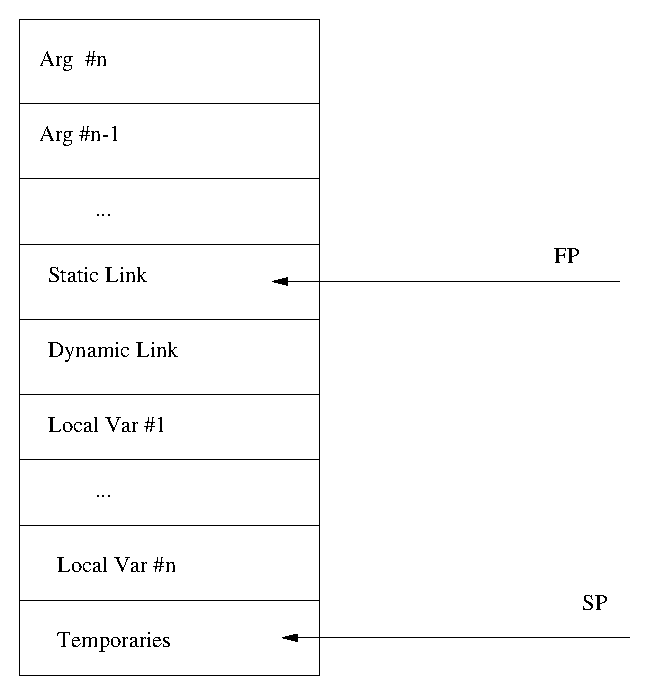
\includegraphics {proc.eps}}
\caption{Stack layout for procedure calls}
\label{fig:proc}
\end{figure}

When a subrotine is called it's arguments are placed in the stack in the left to right order.
This means that the first argument is the deeper one in the stack. After placing the arguments,
the static link is placed in the stack, followed by the dynamic link. The \emph{static link}
contains the address (FP) of the stack frame of the subrotine declared in the previous lexical level.
The \emph{dynamic link} is the previous address of the stack frame (FP). After these actions, space
is allocated to the local variables. The figure \ref{fig:proc} shows the stack frame for a procedure
call. In the figure the stack growns down the page, the bottom of the stack is the first slice.

The frame pointer points to the cell where the static link is placed. When a positive offset is
issued it means a local variable, when it is negative it means an argument.

When a call is made to a routine at the same lexical level that the current one, the static link is
the same that the dynamic link, so the first argument to \keyword{CALL} is 0. If the routine is at a
lower level than the current one then the dynamic link is the same that the current one and the value
of the first argument to \keyword{CALL} is -1. On the other hand if it is a routine at a higher lexical
level than the first argument to \keyword{CALL} is the difference between the levels.

It is the caller responsability to place the stack in the same stack as before the call.

\begin{figure}
\resizebox {10cm}{8cm}{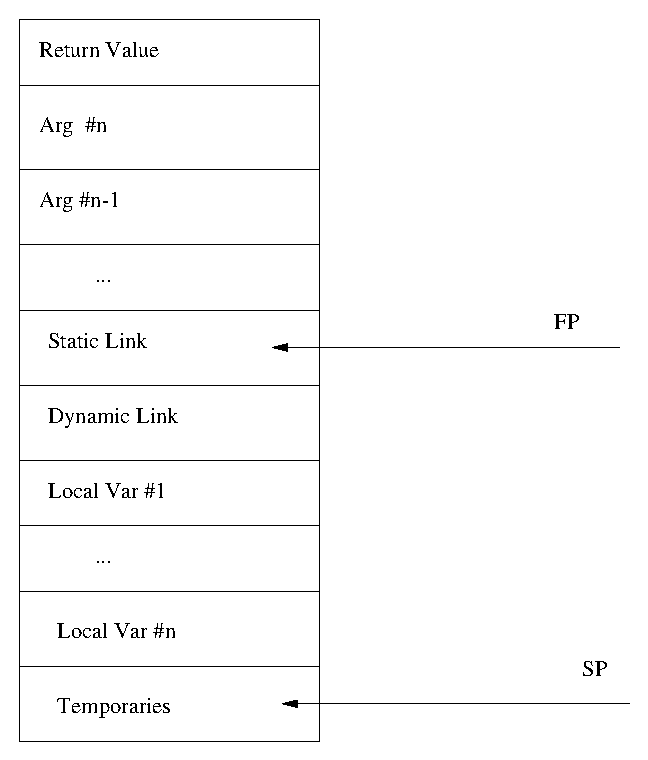
\includegraphics {func.eps}}
\caption{Stack layout for function calls}
\label{fig:func}
\end{figure}

In the case of function calls there isn't a explicit support in LVM, but there is a convention. When calling
a function space is allocated in the stack for the result, so the called routine treats it as an argument
passed by reference. This is displayed in the figure \ref{fig:func}.


\begin{table}[htb]
\center
\begin{tabular}{|c|l|}
 \hline
 Lexical level & Description\\
 \hline\hline
 n $>$ 0 & The called function is n levels above the current one\\ 
 0 & The called function is at the same level that the current one\\
 -1 & The called function is at a lower level\\
 \hline
\end{tabular}
\caption{Lexical levels for computing the CALL instruction}
\label{tbl:levels}
\end{table}

\begin{table}[htb]
\center
\begin{tabular}{|c|l|}
 \hline
 Argument & Routine\\
 \hline\hline
 0 & printint\\ 
 1 & readint\\ 
 2 & printbool\\ 
 3 & readbool\\ 
 4 & println\\ 
 \hline
\end{tabular}
\caption{Codes for standard routines}
\label{tbl:callargs}
\end{table}


\subsection{Arithmetic Operators}

\begin{table}[htb]
 \begin{tabular}{|l|l|}
  \hline
  OpCode & Description\\
  \hline\hline
   ADD & [SP - 1] \arrow{} V1, [SP - 2] \arrow{} V2, SP - 1 \arrow{} SP, V1 + V2 \arrow{} [SP - 1]\\ 
   SUB & [SP - 1] \arrow{} V1, [SP - 2] \arrow{} V2, SP - 1 \arrow{} SP, V1 - V2 \arrow{} [SP - 1]\\  
   MUL & [SP - 1] \arrow{} V1, [SP - 2] \arrow{} V2, SP - 1 \arrow{} SP, V1 * V2 \arrow{} [SP - 1]\\  
   DIV & [SP - 1] \arrow{} V1, [SP - 2] \arrow{} V2, SP - 1 \arrow{} SP, V1 / V2 \arrow{} [SP - 1]\\  
   NEG & [SP - 1] \arrow{} V1, - V1 \arrow{} [SP - 1]\\  
   NOT & [SP - 1] \arrow{} V1,  not V1 \arrow{} [SP - 1]\\  
   AND & [SP - 1] \arrow{} V1, [SP - 2] \arrow{} V2, SP - 1 \arrow{} SP, V1 and V2 \arrow{} [SP - 1]\\  
   OR & [SP - 1] \arrow{} V1, [SP - 2] \arrow{} V2, SP - 1 \arrow{} SP, V1 or V2 \arrow{} [SP - 1]\\  
   EQ & [SP - 1] \arrow{} V1, [SP - 2] \arrow{} V2, SP - 1 \arrow{} SP, V1 = V2 \arrow{} [SP - 1]\\  
   NEQ & [SP - 1] \arrow{} V1, [SP - 2] \arrow{} V2, SP - 1 \arrow{} SP, V1 != V2 \arrow{} [SP - 1]\\  
   LT & [SP - 1] \arrow{} V1, [SP - 2] \arrow{} V2, SP - 1 \arrow{} SP, V1 $<$ V2 \arrow{} [SP - 1]\\  
   GT & [SP - 1] \arrow{} V1, [SP - 2] \arrow{} V2, SP - 1 \arrow{} SP, V1 $>$ V2 \arrow{} [SP - 1]\\  
   GEQ & [SP - 1] \arrow{} V1, [SP - 2] \arrow{} V2, SP - 1 \arrow{} SP, V1 $>$= V2 \arrow{} [SP - 1]\\  
   LEQ & [SP - 1] \arrow{} V1, [SP - 2] \arrow{} V2, SP - 1 \arrow{} SP, V1 $<$= V2 \arrow{} [SP - 1]\\  
 \hline
 \end{tabular}
 \caption{Instructions for performing math operations}
 \label{tbl:mathop}
\end{table}

The table \ref{tbl:mathop} describes the available arithemetic operators in LVM. All the
operators perform 32 bit integer arithemetic. Checking for bad arguments, like \emph{division
by zero} is not required, but advisable. The numbers can be negative, althought there isn't
a standard representation, we think that two's complement is a good choice.

%-------------------------------------------------------------------------
\chapter{Code generation}

The compiler currently offers two backendss

The original backend that was part of the first release, which generates L98 bytecodes,
and a new one that generates 32 bit x86 code.


\section{Generating bytecodes}

By default, the compiler will produce a text file with the \emph{.s} extension,
containing a textual version of the LVM bytecode.


\subsection{Bytecode file format}

  The format is the same used by most assemblers :

\begin{verbatim}
[Label:] instruction [; comment]
\end{verbatim}

  The entry point of the program is specified by the label P$\_$START, and the \keyword{GLOBAL}
instruction needs to be the first in the sequence of instructions.

\section{Generating native code}

To generate an executable, instead of plain bytecode, the compiler needs to be
invoked with the \emph{-e} switch.

In the first release the compilation to native code was performed by making use
of NASM macros that translated the bytecodes text file into x86 Assembly code.

In this release, the backend was refactored and now it takes the responsability
to generate proper Assembly code as well.

Currently an Assembly file is generated in the AT\&T format ending with a \emph{.s}
extension, similar to the bytecode case.

The runtime is still written in C and is stored as a resource inside the \emph{jar}
file.

During compilation to native code, a temporary file with the runtime code is generated
and GCC is invoked with it and the generated Assembly file together.

\section{The builtin routines}

  The builtin routines are defined in C. This makes the compiler dependent on a C
compiler in addition to an Assembler and Linker.

  On the other hand, it allows for more portability across systems, due to the
ways it is possible to invoke kernel APIs across operating systems, regardless of
the process architecture.

  Currently there is the plan to eventually improve the L98 language to be able to
do syscalls, thus removing the need of a C compiler in the process.

%-------------------------------------------------------------------------
\chapter{Installing and using the compiler}

\section{Installing}
  To install the compiler you need to have installed the following software:

\begin{itemize}  
\item a JDK compatible with Java version 7 or higher;
\item Maven version 3 or higher;
\item GNU binutils and GCC (required for native code generation).
\end{itemize}

To compile the compiler, execute the following steps:

\begin{enumerate}
\item \emph{cd} into the L98 directory;
\item Make sure Maven and Java are defined in the \emph{PATH}
\item invoke \emph{mvn}
\end{enumerate}

  Assuming everything went without errors you can start using the L98 compiler.

\section{Compiling}
  To compile your programs, you just have to use the \emph{l98c} shell script.
The \emph{l98c} command is a sh shell script. It invokes the java interpreter
with the name of the class that implements the compiler and the program arguments.

The command line sintax for invoking the \emph{l98c}script is :

\begin{verbatim}
  l98c aSourceFile.l98
\end{verbatim}

This way an \emph{aSourceFile.s} file is created with the LVM code. If the
\switch{-e} switch additionally given, the contains x86 code.

\begin{verbatim}
  l98c -e aSourceFile.l98
\end{verbatim}

An executable file named \emph{aSourceFile} is generated.

If you want the intermediate Assembly file to be left on the system, you should
use the \switch{-s} switch as well.


%-------------------------------------------------------------------------
\chapter{License}

 This release is under the GNU GPL v2.

%-------------------------------------------------------------------------

\begin{thebibliography}{1}
\bibitem{tiger}{Addrew W. Appel. \textsl{Modern Compiler Implementation in Java}. 1998 Cambridge University Press. ISBN 0521583888}
\end{thebibliography}

\end{document}




